\section{Développement}

    \subsection{Chiffrement d'une image}

        \begin{frame}
            \frametitle{Chiffrement par mélange pseudo-aléatoire}
            \centering{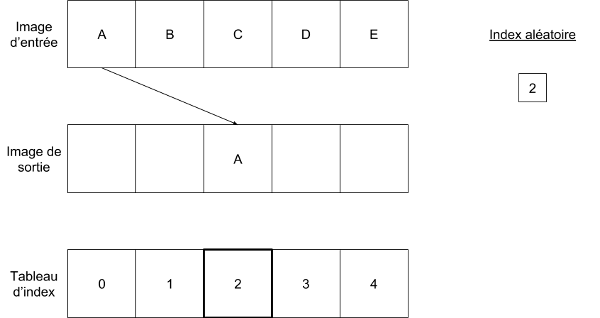
\includegraphics[width=.5\linewidth]{./rsc/index_1_1.png}}
            \pause
            \begin{columns}
                \begin{column}{.45\linewidth}
                    \centering{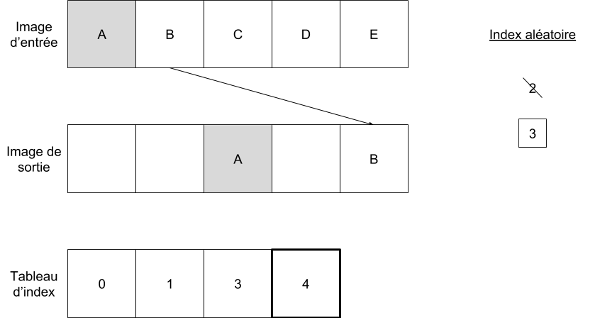
\includegraphics[width=\linewidth]{./rsc/index_1_2.png}}
                \end{column}
                \pause
                \begin{column}{.45\linewidth}
                    \centering{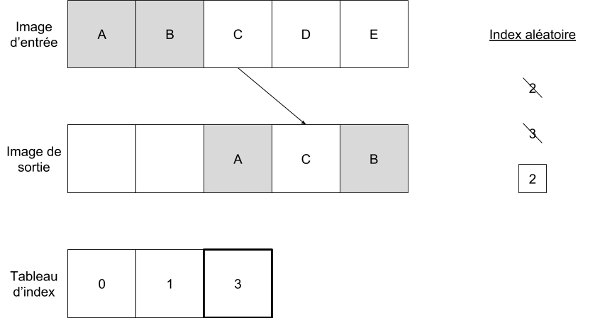
\includegraphics[width=\linewidth]{./rsc/index_1_3.png}}
                \end{column}
            \end{columns}
        \end{frame}

        \begin{frame}
            \frametitle{Chiffrement par mélange pseudo-aléatoire}
            \framesubtitle{Résultats}
            \begin{columns}
                \begin{column}{.5\linewidth}
                    \centering{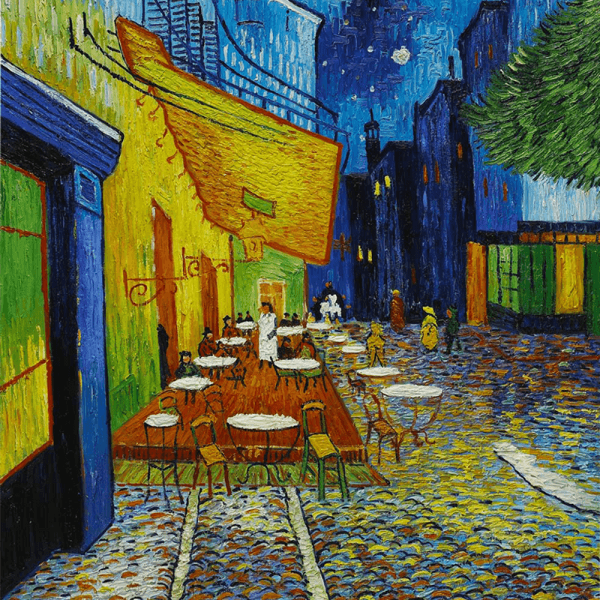
\includegraphics[width=\linewidth]{./rsc/van_gogh.png}}
                    \centering{"Terrasse du café le soir", Van Gogh}
                \end{column}

                \begin{column}{.5\linewidth}
                    \centering{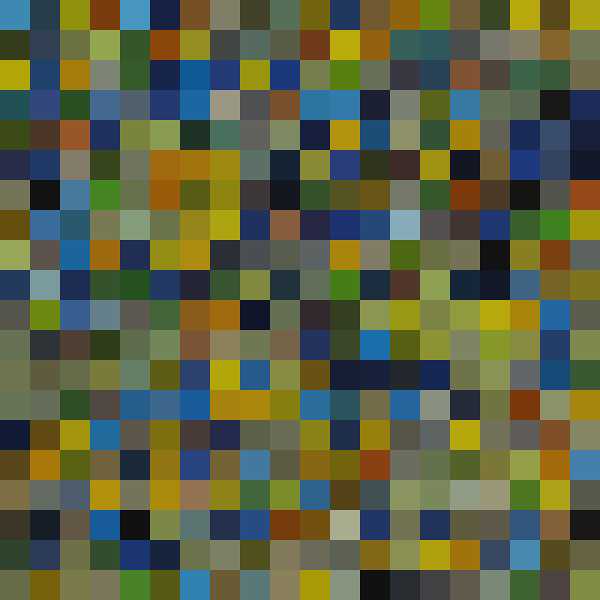
\includegraphics[width=\linewidth]{./rsc/van_gogh_40.png}}
                    \centering{Peinture chiffrée avec des blocs de 20x20 pixels}
                \end{column}
            \end{columns}
        \end{frame}

        \begin{frame}
            \frametitle{Déchiffrement par mélange pseudo-aléatoire}
            \centering{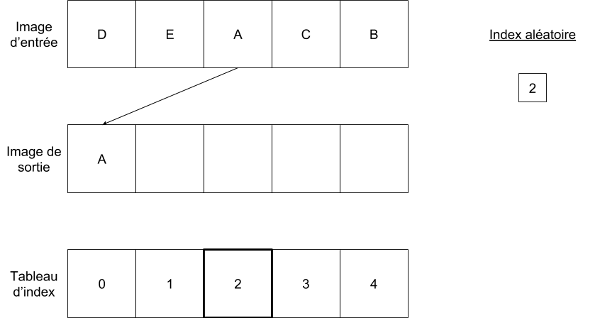
\includegraphics[width=.5\linewidth]{./rsc/index_2_1.png}}
            \pause
            \begin{columns}
                \begin{column}{.45\linewidth}
                    \centering{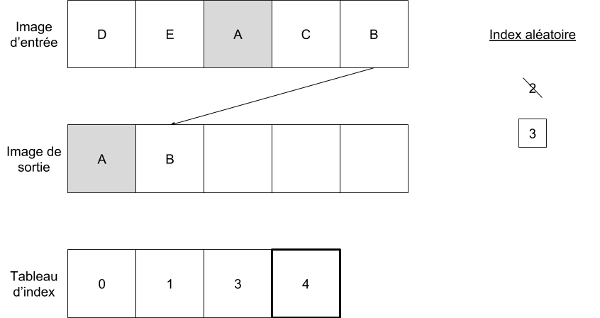
\includegraphics[width=\linewidth]{./rsc/index_2_2.png}}
                \end{column}
                \pause
                \begin{column}{.45\linewidth}
                    \centering{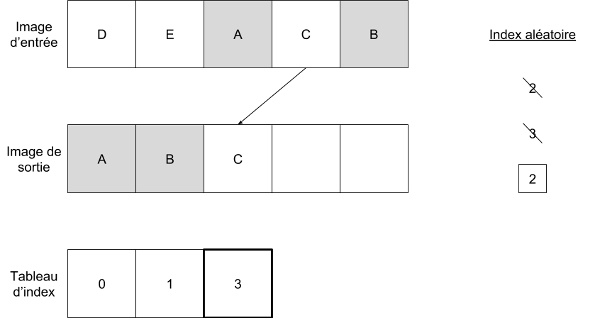
\includegraphics[width=\linewidth]{./rsc/index_2_3.png}}
                \end{column}
            \end{columns}
        \end{frame}

    \subsection{Lecture d'une image}

        \begin{frame}
            \frametitle{Prétraitement}
            \framesubtitle{Niveaux de gris / Binaire}
            \begin{columns}
                \begin{column}{.3\linewidth}
                    \centering{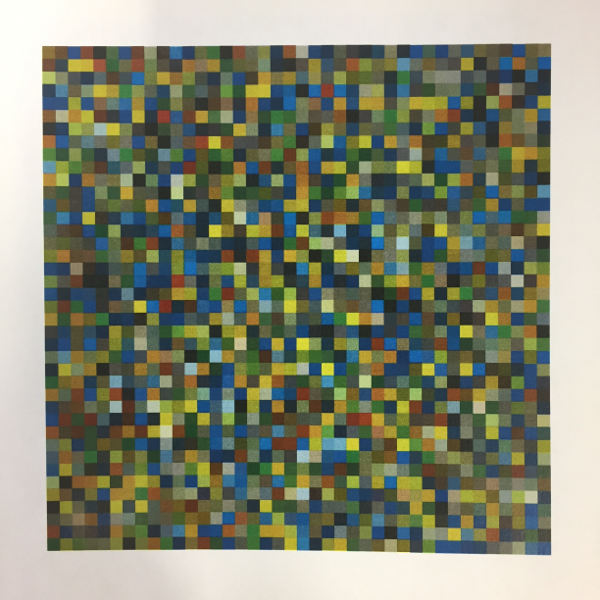
\includegraphics[width=\linewidth]{./rsc/40.png}}
                \end{column}
                \begin{column}{.3\linewidth}
                    \centering{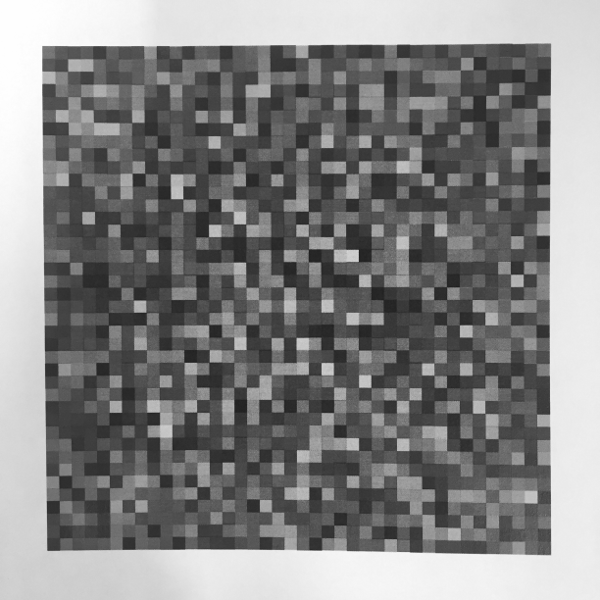
\includegraphics[width=\linewidth]{./rsc/gray_scale.png}}
                \end{column}
                \begin{column}{.3\linewidth}
                    \centering{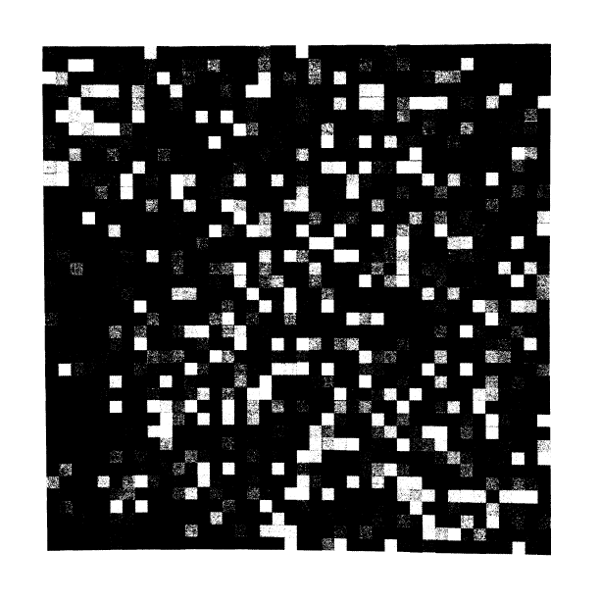
\includegraphics[width=\linewidth]{./rsc/binary.png}}
                \end{column}
            \end{columns}
            \pause
            \begin{exampleblock}{Équation niveaux de gris}
                \centering{$0.299 \cdot Rouge + 0.587 \cdot Vert + 0.144 \cdot Bleu$}
            \end{exampleblock}
            \begin{exampleblock}{Seuil de conversion binaire}
                \centering{$seuil = \frac{\sum_{i = 0}^{m \cdot n} X{i}}{m \cdot n}$}
            \end{exampleblock}
        \end{frame}

        \begin{frame}
            \frametitle{Prétraitement}
            \framesubtitle{Détection des angles / Transformation}
            \begin{columns}
                \begin{column}{.3\linewidth}
                    \centering{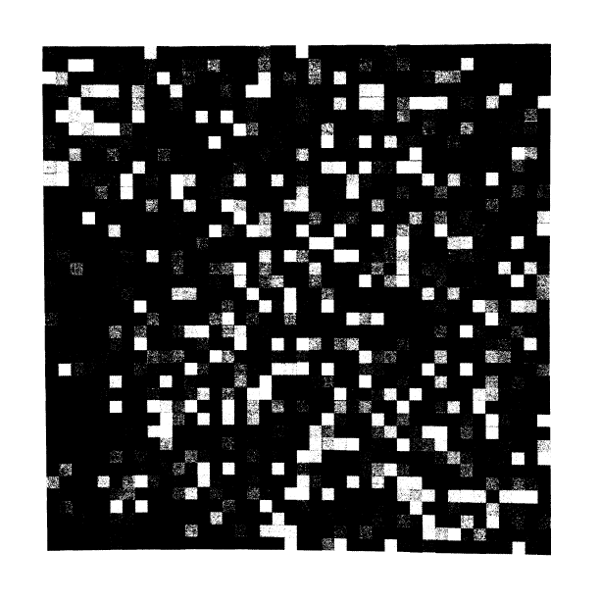
\includegraphics[width=\linewidth]{./rsc/binary.png}}
                \end{column}
                \begin{column}{.3\linewidth}
                    \centering{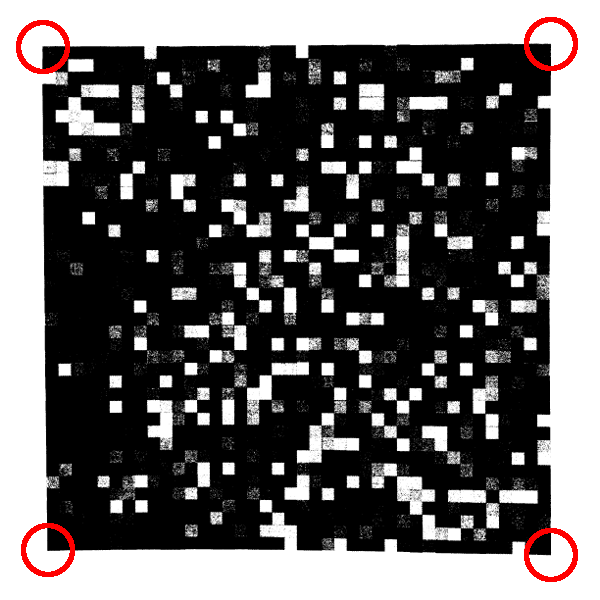
\includegraphics[width=\linewidth]{./rsc/angles.png}}
                \end{column}
                \begin{column}{.3\linewidth}
                    \centering{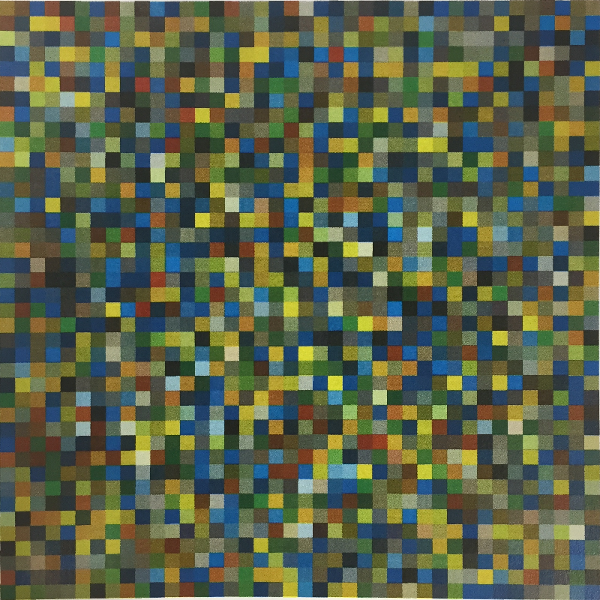
\includegraphics[width=\linewidth]{./rsc/transform.png}}
                \end{column}
            \end{columns}
            \pause
            \begin{exampleblock}{Détection des angles}
                \centering{$angle_{top,right} = X_{ij}, min(\sqrt{(0-i)^{2} + (width-j)^{2}})$}
            \end{exampleblock}
            \begin{exampleblock}{Transformation affine et interpolation}
                \centering{A, B, C et D : les 4 angles de la peinture}\\
                \centering{E, F, G et H : les pts évoluant (resp.) sur AB, BC, CD et AD}\\
                \centering{K : l'intersection de EG et FH}
            \end{exampleblock}
        \end{frame}

        \begin{frame}
            \frametitle{Déchiffrement}
            \begin{columns}
                \begin{column}{.45\linewidth}
                    \centering{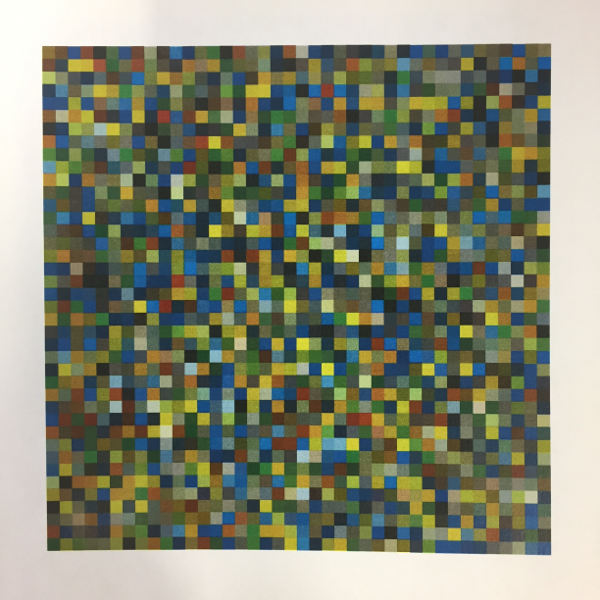
\includegraphics[width=\linewidth]{./rsc/40.png}}
                \end{column}
                \pause
                \begin{column}{.45\linewidth}
                    \centering{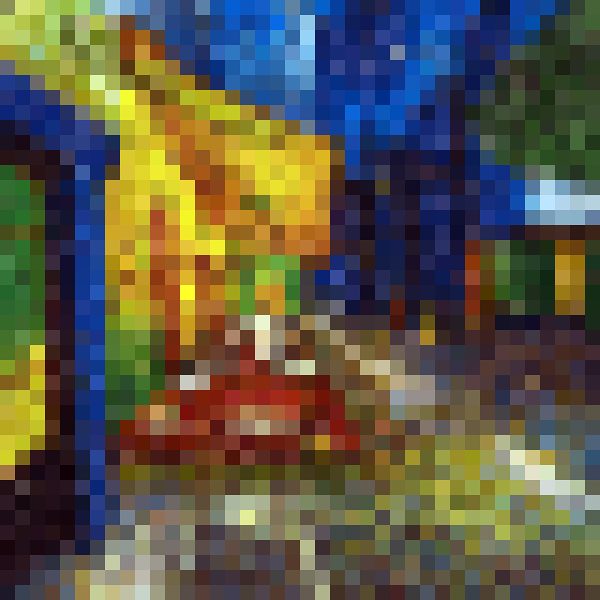
\includegraphics[width=\linewidth]{./rsc/decrypt.png}}
                \end{column}
            \end{columns}
        \end{frame}

    \subsection{Analyse des résultats}

        \begin{frame}
            \frametitle{PSNR découpage en bloc}
            \centering{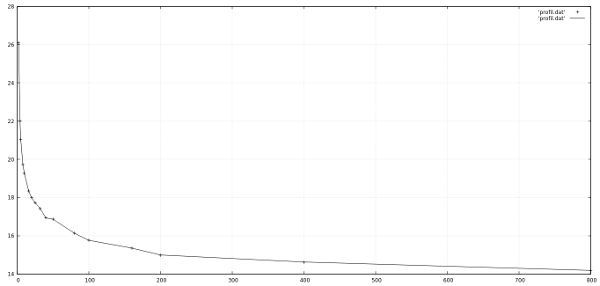
\includegraphics[width=.8\linewidth]{./rsc/psnr_ressemblance.png}}\\
            \centering{PSNR d'une image en fonction de la taille des blocs}
        \end{frame}

        \begin{frame}
            \frametitle{PSNR lecture et déchiffrement}
            \centering{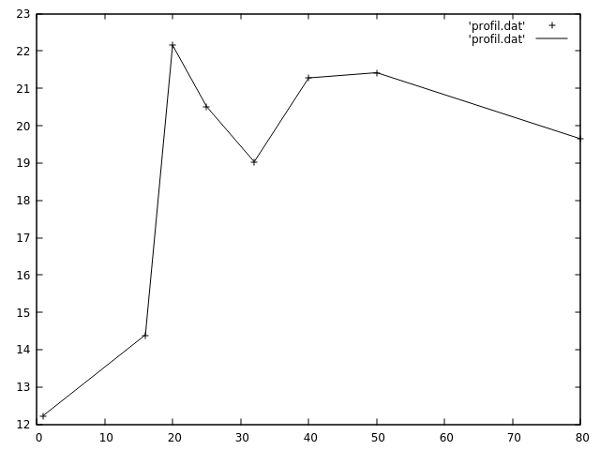
\includegraphics[width=.8\linewidth]{./rsc/psnr_lecture.png}}\\
            \centering{PSNR d'une image déchiffrée en fonction de la taille des blocs}
        \end{frame}

    \subsection{Portage sous mobile}

        \begin{frame}
            \frametitle{Portage sous mobile}
            \framesubtitle{Choix de l'outil}
            \begin{columns}
                \begin{column}{.45\linewidth}
                    \centering{
\includegraphics[width=.7\linewidth]{./rsc/logo_native_script.png}}
                \end{column}
                \begin{column}{.45\linewidth}
                    \centering{
\includegraphics[width=.8\linewidth]{./rsc/logo_android_studio.png}}
                \end{column}
            \end{columns}

            \begin{columns}
                \begin{column}{.45\linewidth}
                    \centering{
\includegraphics[width=.9\linewidth]{./rsc/logo_ionic.png}}
                \end{column}
                \begin{column}{.45\linewidth}
                    \centering{
\includegraphics[width=.8\linewidth]{./rsc/logo_react_native.png}}
                \end{column}
            \end{columns}
        \end{frame}

        \begin{frame}
            \frametitle{Portage sous mobile}
            \framesubtitle{Choix de l'outil}
            \centering{
\includegraphics[width=.7\linewidth]{./rsc/logo_ionic.png}}
            \begin{block}{Différentes possibilités}
                \begin{itemize}
                    \item Utilisation de la bibliothèque OpenCV Javascript.
                    \item Interprétation du code C++ dans l'application.
                    \item Traitement sur un serveur.
                \end{itemize}
            \end{block}
        \end{frame}

        \begin{frame}
            \frametitle{Portage sous mobile}
            \framesubtitle{Choix de l'outil}
            \begin{columns}
                \begin{column}{.33\linewidth}
                    \centering{
\includegraphics[width=.7\linewidth]{./rsc/logo_raspberry.png}}
                \end{column}
                \begin{column}{.33\linewidth}
                    \centering{
\includegraphics[width=\linewidth]{./rsc/logo_ionic.png}}
                \end{column}
                \begin{column}{.33\linewidth}
                    \centering{
\includegraphics[width=.8\linewidth]{./rsc/logo_node_js.png}}
                \end{column}
            \end{columns}
        \end{frame}

        \begin{frame}
            \frametitle{Portage sous mobile}
            \framesubtitle{Première implémentation}
            \begin{columns}
                \begin{column}{.33\linewidth}
                    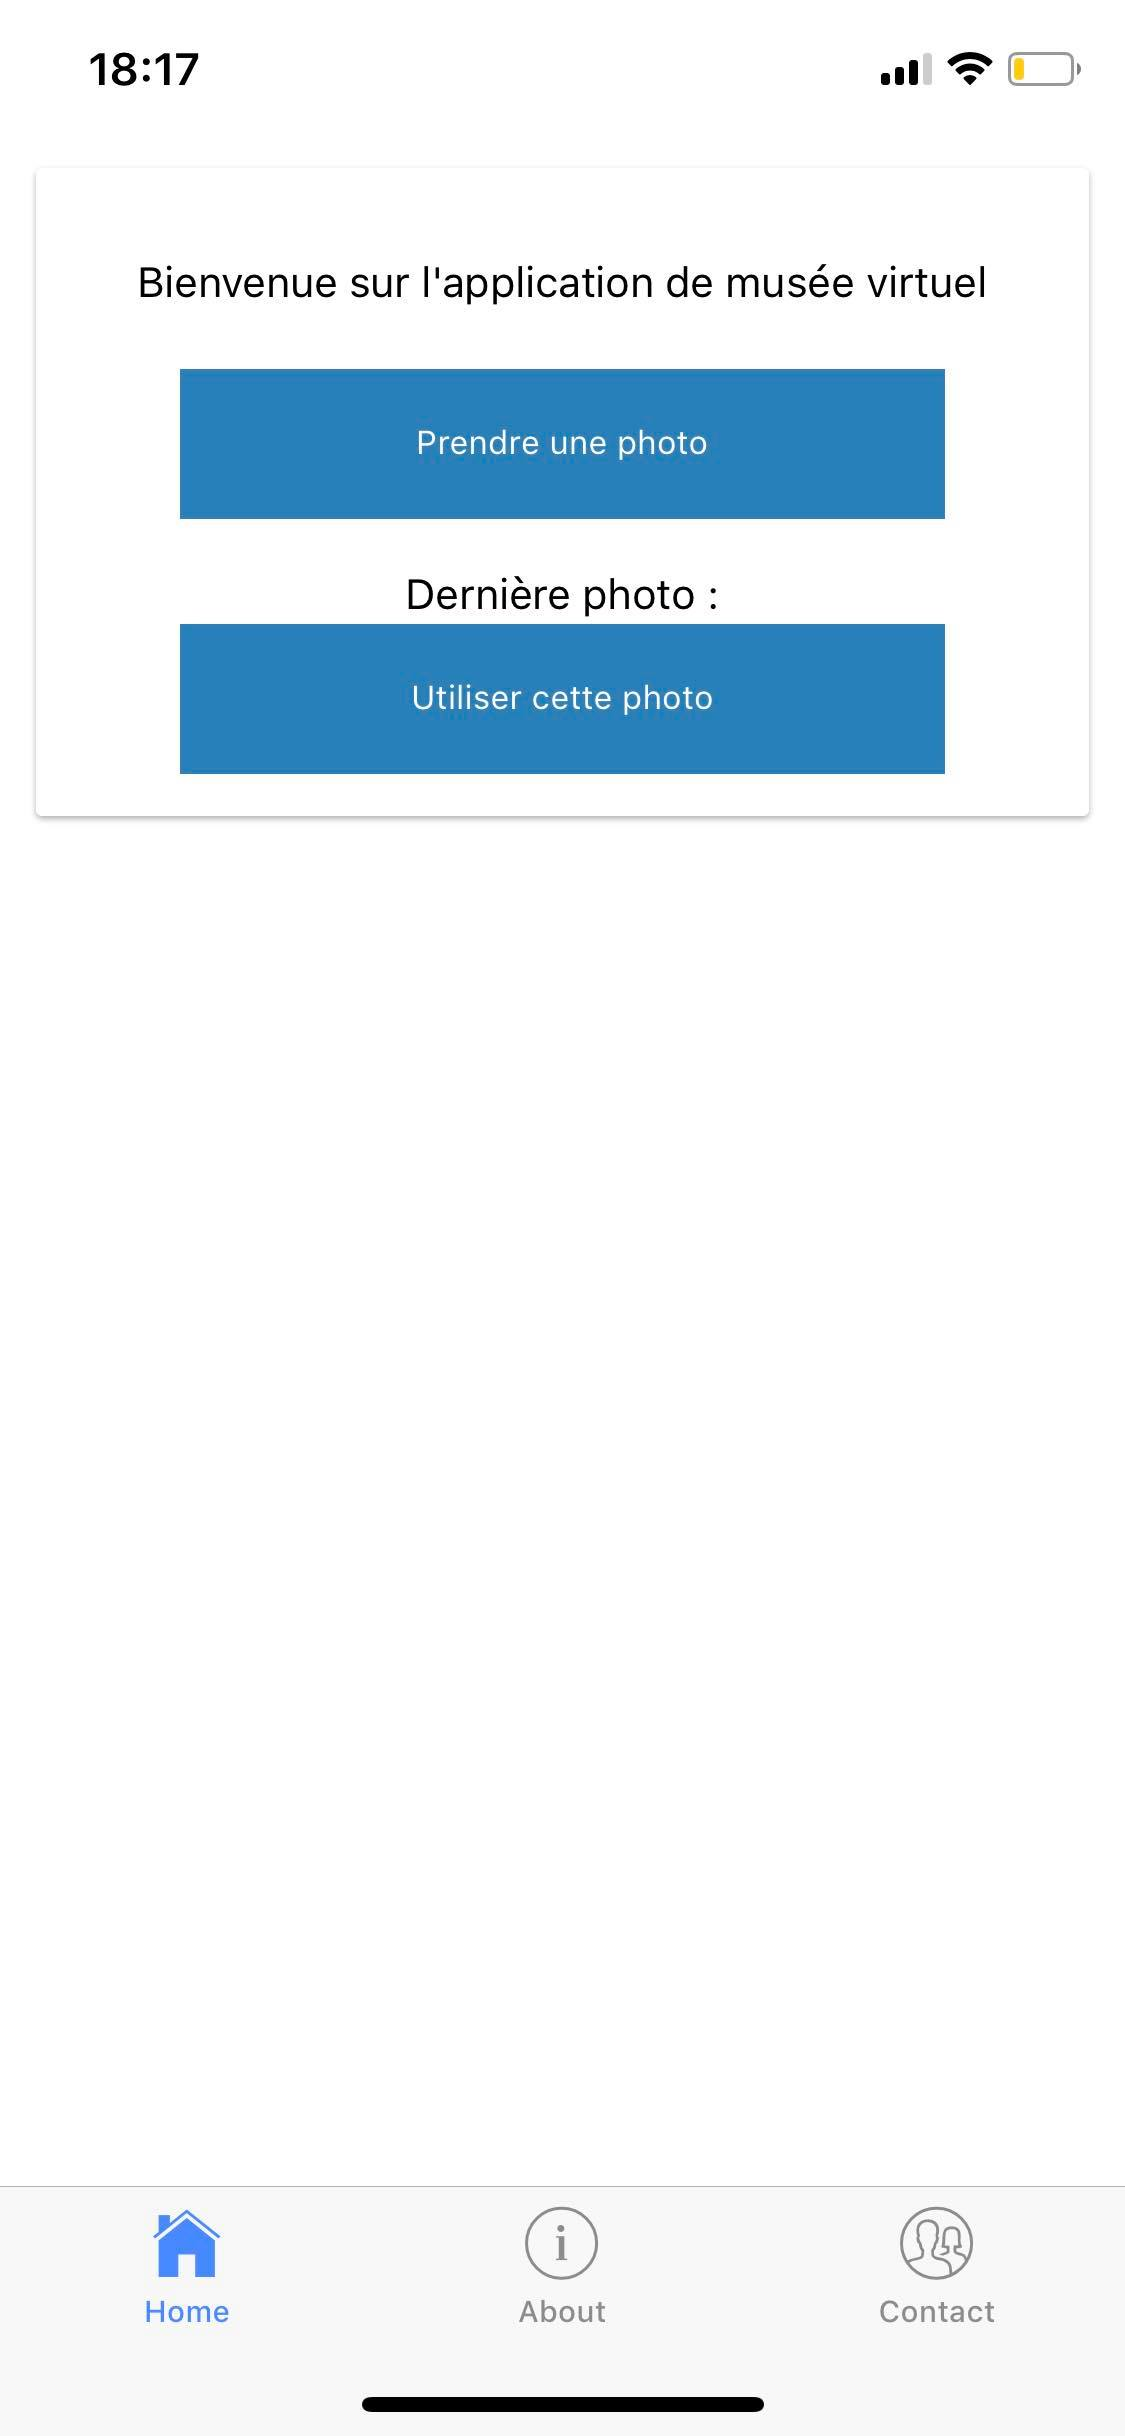
\includegraphics[width=\linewidth]{./rsc/appli_1.png}
                \end{column}
                \begin{column}{.33\linewidth}
                    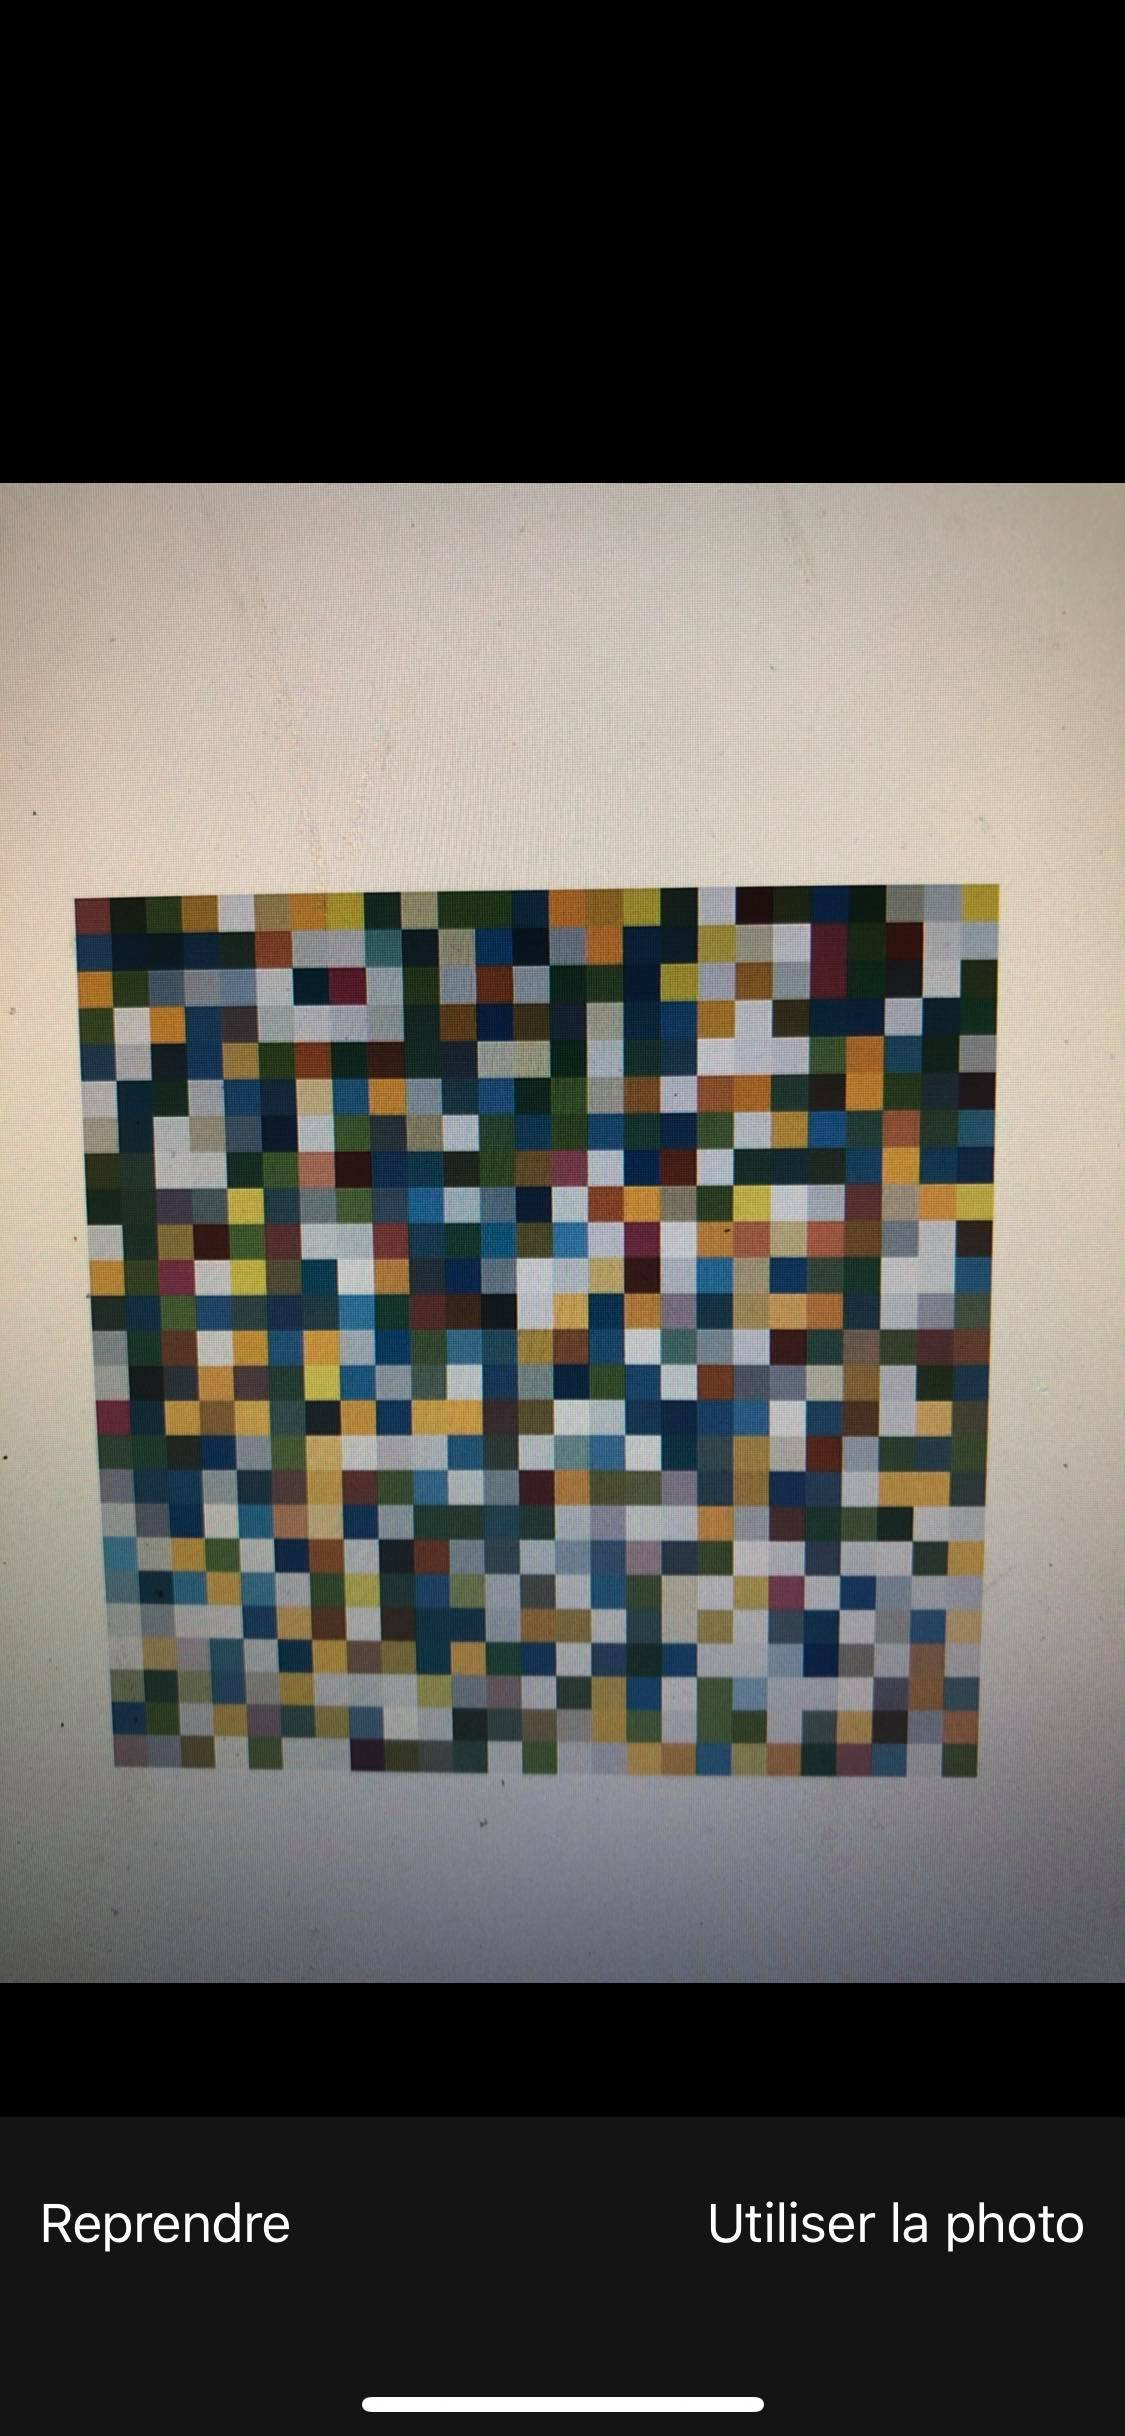
\includegraphics[width=\linewidth]{./rsc/appli_2.png}
                \end{column}
                \begin{column}{.33\linewidth}
                    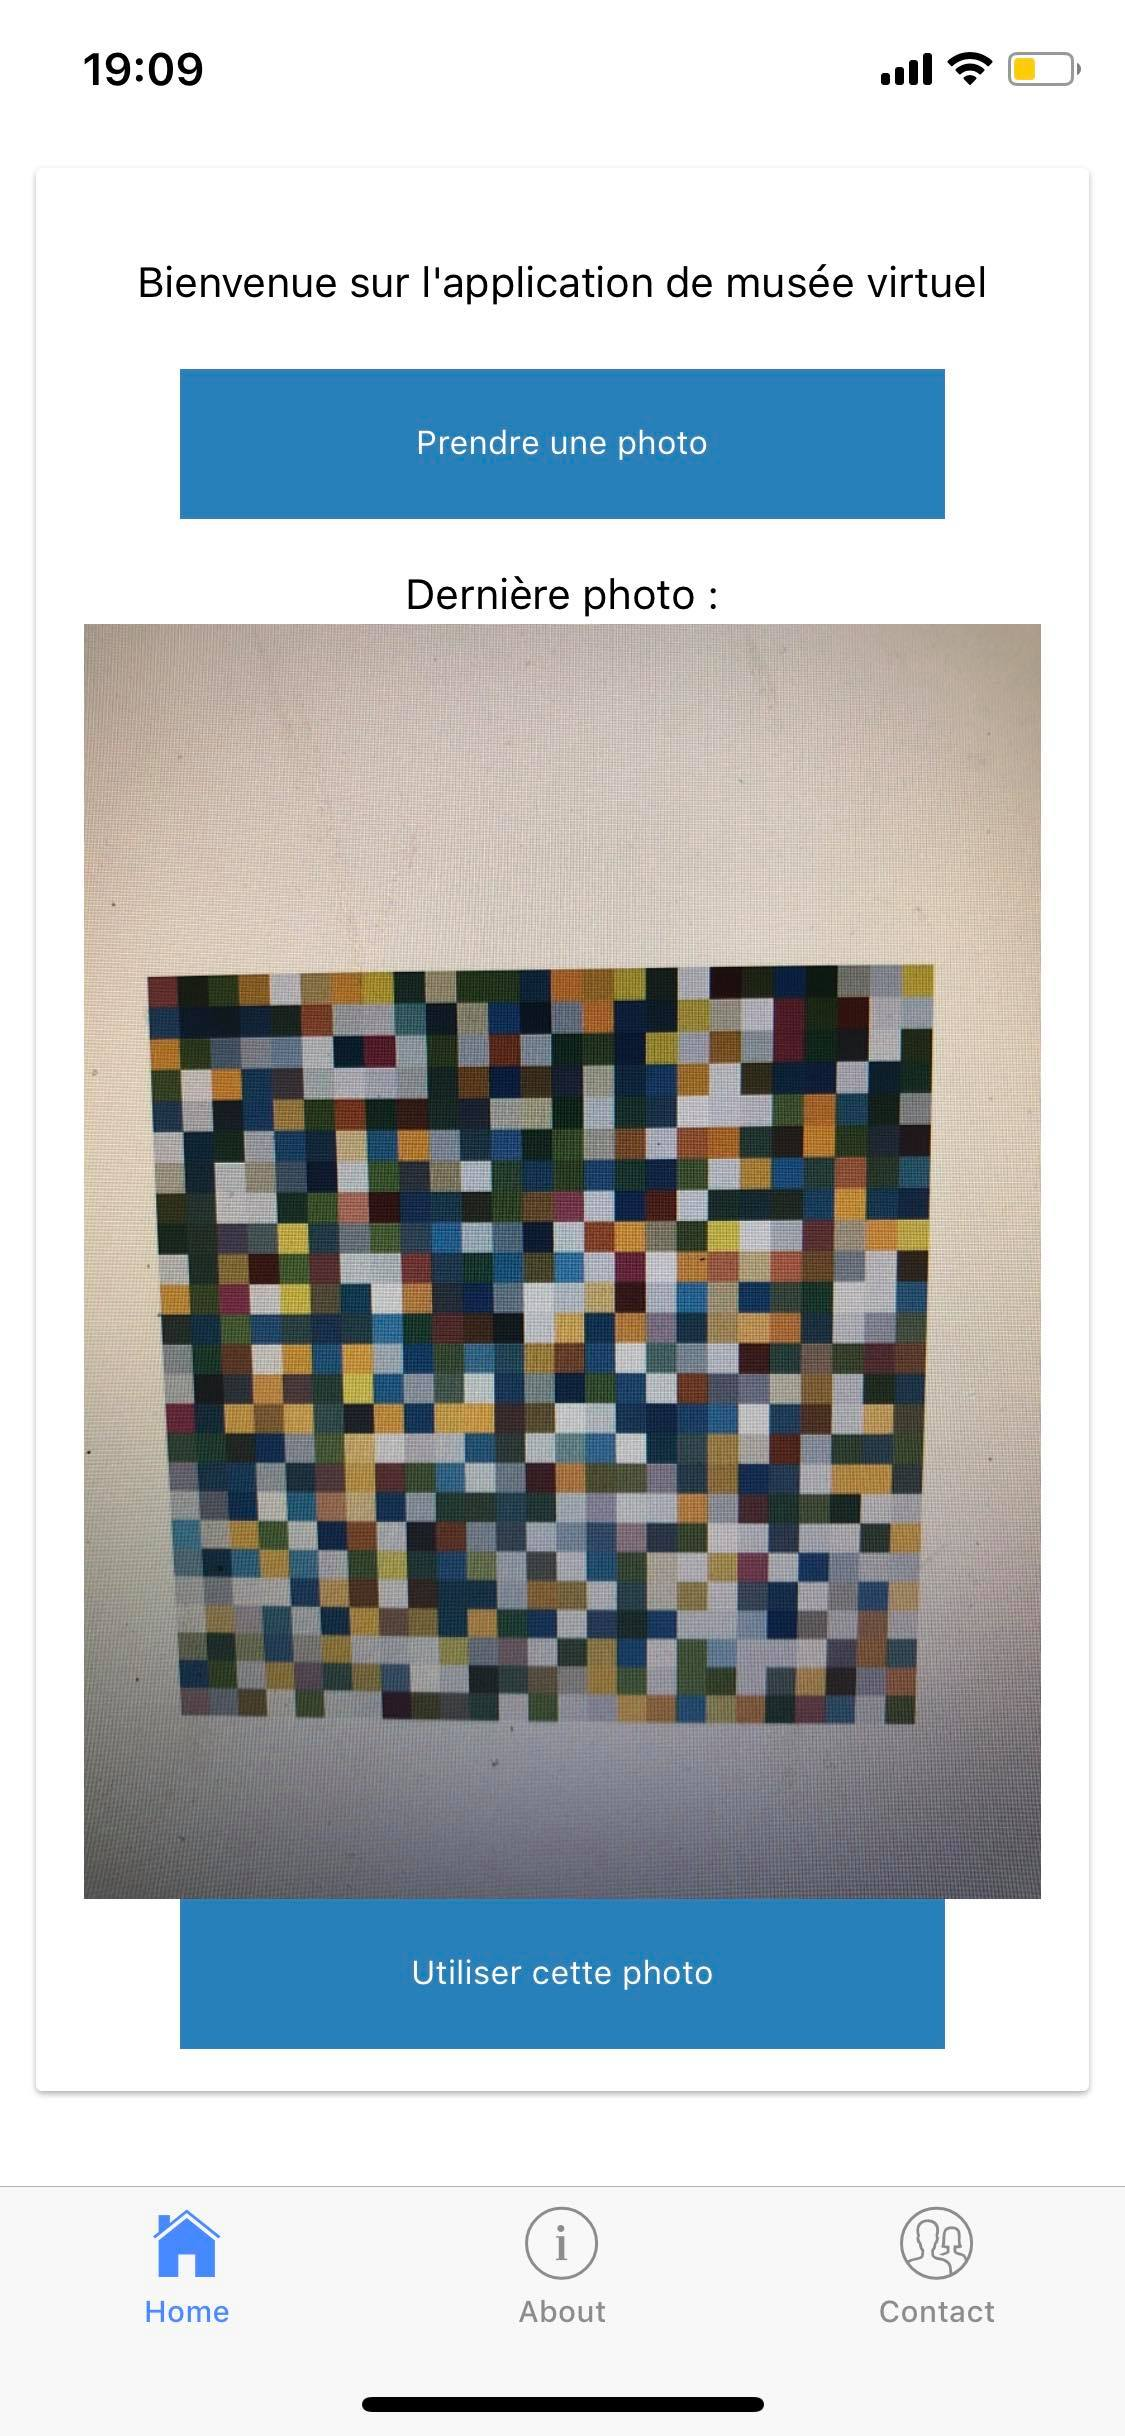
\includegraphics[width=\linewidth]{./rsc/appli_3.png}
                \end{column}
            \end{columns}
        \end{frame}
